\section{Method}
\label{sec:method}

We keep the \sea gate of \seacache and change what is written on skipped steps (\cref{fig:method}). We review
flow-matching sampling, residual caching and the gate (\cref{sec:prelim}), then describe the Kalman predictor
(\cref{sec:kalman}), the corrector \pcgs (\cref{sec:pcgs}) and the cost (\cref{sec:cost}).

% Method figure (figures/method.pdf, built from figures/src/method/). The caption is generated by the figure agent
% (figures/method_caption.tex, \label{fig:method}); the fallback below is used only if that file is missing.
\begin{figure*}[t]
  \centering
  \maybegraphics[width=\textwidth]{figures/method.pdf}
  \IfFileExists{figures/method_caption.tex}{% Draft caption for the method figure (Fig. 2).  Usage in sections/method.tex:
%   \begin{figure*}[t]\centering
%     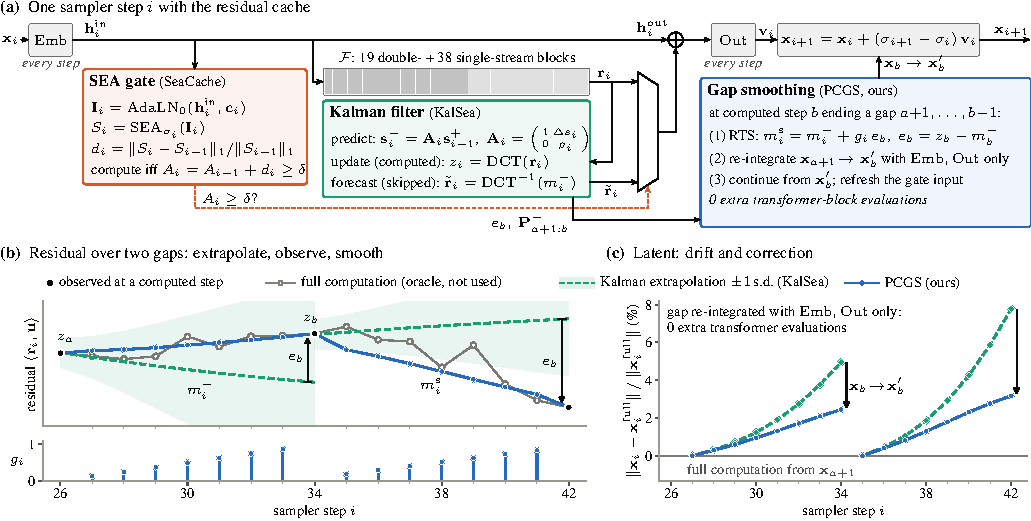
\includegraphics[width=\textwidth]{figures/method.pdf}
%     % Draft caption for the method figure (Fig. 2).  Usage in sections/method.tex:
%   \begin{figure*}[t]\centering
%     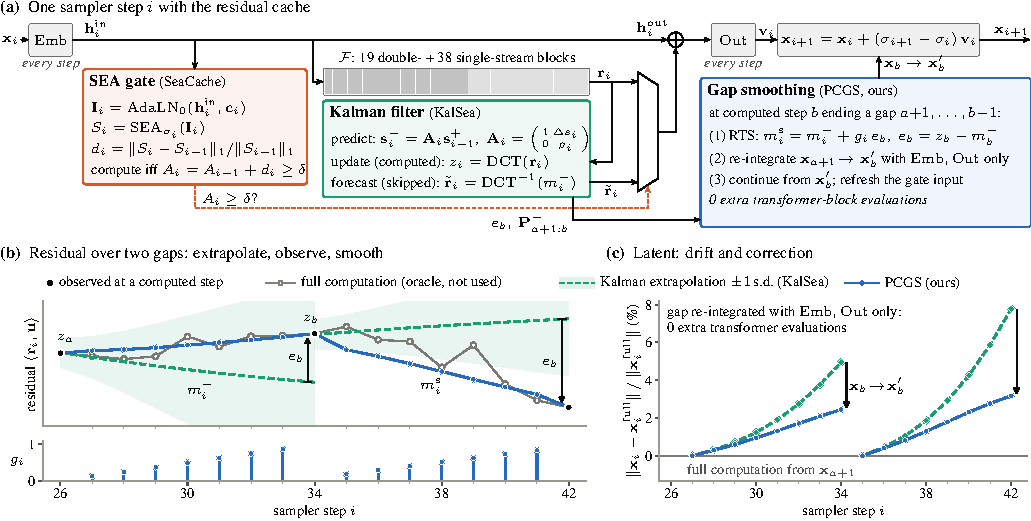
\includegraphics[width=\textwidth]{figures/method.pdf}
%     % Draft caption for the method figure (Fig. 2).  Usage in sections/method.tex:
%   \begin{figure*}[t]\centering
%     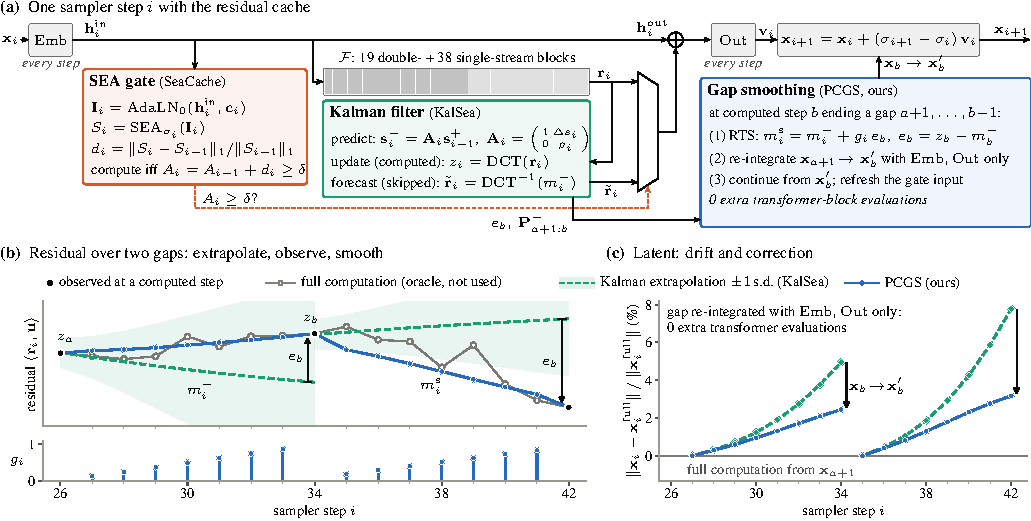
\includegraphics[width=\textwidth]{figures/method.pdf}
%     \input{figures/method_caption}
%   \end{figure*}
% Source and data: figures/src/method/ (build.sh).  Numbers below come from data/method_trace_summary.json
% (one real FLUX.1-dev generation, DrawBench prompt index 154, delta = 0.6, seed = 154).  Steps are 1-based (i = 1..N).
\caption{\textbf{Overview.}
\textbf{(a)}~In each sampler step~$i$, the \sea gate of \seacache accumulates the \sea-filtered relative $\ell_1$ change
$\gdist_i$ of the first block's modulated input and runs the transformer blocks $\blocks$ only when the accumulated change
reaches~$\delta$ (which resets it); the residual $\res_i=\blocks(\hin_i)-\hin_i$ of a computed step updates a damped-trend
Kalman filter per DCT coefficient (\kalsea), whose forecast $\resf_i$ replaces $\res_i$ on skipped steps, while $\Emb$
and $\Out$ run at every step.
\textbf{(b)}~When a computed step~$b$ ends the gap $a{+}1,\dots,b{-}1$, \pcgs propagates the innovation $e_b$ back into
the gap with the RTS gains $g_i$, which grow toward~$b$, so that the smoothed residuals $\smooth{m}_i$ replace the
extrapolation $\prior{m}_i$.
\textbf{(c)}~The gap is then re-integrated from $\lat_{a+1}$ with $\Emb$ and $\Out$ only and sampling continues from $\lat_b'$,
which roughly halves the latent deviation from full computation at~$b$ (here $5.0\%\to2.4\%$ and $7.8\%\to3.2\%$;
25--59\% lower in all ten gaps of this sample) at zero extra transformer evaluations.
Panels (b) and (c) show one real \flux generation at $\delta=0.6$ (13 of 50 steps computed) for the DrawBench prompt
whose PSNR gains (\kalsea over \seacache, \ours over \kalsea) are closest to the benchmark means (``McDonalds Church.'');
the residual is projected onto a fixed random unit direction~$\mathbf{u}$ in the lowest DCT band, which holds 89\% of the
residual energy, and the gray full-computation values come from extra evaluations made only for this figure.}
\label{fig:method}

%   \end{figure*}
% Source and data: figures/src/method/ (build.sh).  Numbers below come from data/method_trace_summary.json
% (one real FLUX.1-dev generation, DrawBench prompt index 154, delta = 0.6, seed = 154).  Steps are 1-based (i = 1..N).
\caption{\textbf{Overview.}
\textbf{(a)}~In each sampler step~$i$, the \sea gate of \seacache accumulates the \sea-filtered relative $\ell_1$ change
$\gdist_i$ of the first block's modulated input and runs the transformer blocks $\blocks$ only when the accumulated change
reaches~$\delta$ (which resets it); the residual $\res_i=\blocks(\hin_i)-\hin_i$ of a computed step updates a damped-trend
Kalman filter per DCT coefficient (\kalsea), whose forecast $\resf_i$ replaces $\res_i$ on skipped steps, while $\Emb$
and $\Out$ run at every step.
\textbf{(b)}~When a computed step~$b$ ends the gap $a{+}1,\dots,b{-}1$, \pcgs propagates the innovation $e_b$ back into
the gap with the RTS gains $g_i$, which grow toward~$b$, so that the smoothed residuals $\smooth{m}_i$ replace the
extrapolation $\prior{m}_i$.
\textbf{(c)}~The gap is then re-integrated from $\lat_{a+1}$ with $\Emb$ and $\Out$ only and sampling continues from $\lat_b'$,
which roughly halves the latent deviation from full computation at~$b$ (here $5.0\%\to2.4\%$ and $7.8\%\to3.2\%$;
25--59\% lower in all ten gaps of this sample) at zero extra transformer evaluations.
Panels (b) and (c) show one real \flux generation at $\delta=0.6$ (13 of 50 steps computed) for the DrawBench prompt
whose PSNR gains (\kalsea over \seacache, \ours over \kalsea) are closest to the benchmark means (``McDonalds Church.'');
the residual is projected onto a fixed random unit direction~$\mathbf{u}$ in the lowest DCT band, which holds 89\% of the
residual energy, and the gray full-computation values come from extra evaluations made only for this figure.}
\label{fig:method}

%   \end{figure*}
% Source and data: figures/src/method/ (build.sh).  Numbers below come from data/method_trace_summary.json
% (one real FLUX.1-dev generation, DrawBench prompt index 154, delta = 0.6, seed = 154).  Steps are 1-based (i = 1..N).
\caption{\textbf{Overview.}
\textbf{(a)}~In each sampler step~$i$, the \sea gate of \seacache accumulates the \sea-filtered relative $\ell_1$ change
$\gdist_i$ of the first block's modulated input and runs the transformer blocks $\blocks$ only when the accumulated change
reaches~$\delta$ (which resets it); the residual $\res_i=\blocks(\hin_i)-\hin_i$ of a computed step updates a damped-trend
Kalman filter per DCT coefficient (\kalsea), whose forecast $\resf_i$ replaces $\res_i$ on skipped steps, while $\Emb$
and $\Out$ run at every step.
\textbf{(b)}~When a computed step~$b$ ends the gap $a{+}1,\dots,b{-}1$, \pcgs propagates the innovation $e_b$ back into
the gap with the RTS gains $g_i$, which grow toward~$b$, so that the smoothed residuals $\smooth{m}_i$ replace the
extrapolation $\prior{m}_i$.
\textbf{(c)}~The gap is then re-integrated from $\lat_{a+1}$ with $\Emb$ and $\Out$ only and sampling continues from $\lat_b'$,
which roughly halves the latent deviation from full computation at~$b$ (here $5.0\%\to2.4\%$ and $7.8\%\to3.2\%$;
25--59\% lower in all ten gaps of this sample) at zero extra transformer evaluations.
Panels (b) and (c) show one real \flux generation at $\delta=0.6$ (13 of 50 steps computed) for the DrawBench prompt
whose PSNR gains (\kalsea over \seacache, \ours over \kalsea) are closest to the benchmark means (``McDonalds Church.'');
the residual is projected onto a fixed random unit direction~$\mathbf{u}$ in the lowest DCT band, which holds 89\% of the
residual energy, and the gray full-computation values come from extra evaluations made only for this figure.}
\label{fig:method}
}{%
  \caption{\textbf{Overview of \ours.} \textbf{(a)}~One sampler step of a diffusion transformer with a residual cache.
    The input embedding $\Emb$ and the output layers $\Out$ run at every step. The \sea gate of
    \seacache~\cite{chung2026seacache} decides whether the block stack $\blocks$ runs. On computed steps the block-stack
    residual $\res_i$ updates a damped-trend Kalman filter; on skipped steps the filter's forecast replaces it.
    \textbf{(b)}~Predictor-corrector gap smoothing (\pcgs). When step $b$ is computed after the skipped steps
    $a{+}1,\dots,b{-}1$, the innovation $e_b$ (observed minus forecast residual) is distributed over the gap with the
    Rauch--Tung--Striebel smoother gains $g_i$, the gap is re-integrated with $\Emb$ and $\Out$ only, and sampling
    continues from the corrected latent $\lat'_b$. \pcgs adds no transformer evaluations.}
  \label{fig:method}}
\end{figure*}

\subsection{Preliminaries}
\label{sec:prelim}

\paragraph{Flow-matching sampling.}
Rectified-flow models~\cite{liu2023rectifiedflow,lipman2023flow,albergo2023interpolants,esser2024scaling} interpolate
$\lat_\sigma=(1-\sigma)\lat^\star+\sigma\boldsymbol\epsilon$ between data $\lat^\star$ and Gaussian noise
$\boldsymbol\epsilon$, and learn the velocity $\boldsymbol\epsilon-\lat^\star$. Sampling integrates the learned
velocity over a decreasing schedule $\sigma_0>\sigma_1>\dots>\sigma_N=0$ with Euler steps,
\begin{equation}
  \lat_{i+1}=\lat_i+(\sigma_{i+1}-\sigma_i)\,\vel_i,\qquad i=0,\dots,N-1.
  \label{eq:euler}
\end{equation}

\paragraph{Residual caching.}
A diffusion transformer computes the velocity in three stages,
\begin{equation}
  \hin_i=\Emb(\lat_i),\quad \hout_i=\blocks(\hin_i),\quad \vel_i=\Out(\hout_i,\cond_i),
  \label{eq:dit}
\end{equation}
where $\Emb$ embeds the latent patches, $\blocks$ is the block stack (in \flux, 19 double-stream and 38
single-stream blocks, which also process the text tokens), $\Out$ is the final adaptive normalization and linear
projection, and $\cond_i$ embeds the timestep and the guidance scale. Almost all computation is in $\blocks$.
Residual caches~\cite{liu2025teacache,chung2026seacache} store the block-stack residual of the image tokens,
$\res_i=\hout_i-\hin_i$, on computed steps. On skipped steps they run only $\Emb$ and $\Out$, with
$\hout_i=\hin_i+\hat\res_i$, where the filler $\hat\res_i$ is the last computed residual (reuse) or a forecast.

\paragraph{The \sea gate.}
TeaCache~\cite{liu2025teacache} and \seacache~\cite{chung2026seacache} decide whether to compute from the
timestep-modulated input of the first block, $\modin_i$, \ie, its adaptive layer normalization applied to $\hin_i$.
\seacache filters $\modin_i$ on the token grid with the normalized gain of the optimal linear denoiser under a
power-law spectrum, $G_i(f)\propto a_iS(f)/(a_i^2S(f)+b_i^2)$ with $S(f)=|f|^{-\beta}$, $a_i=1-\sigma_i$ and
$b_i=\sigma_i$, and accumulates the relative $\ell_1$ change of the filtered input,
\begin{equation}
  \gdist_i=\frac{\|\seaop_i(\modin_i)-\seaop_{i-1}(\modin_{i-1})\|_1}{\|\seaop_{i-1}(\modin_{i-1})\|_1},
  \quad D_i=D_{i-1}+\gdist_i.
  \label{eq:sea}
\end{equation}
Step $i$ is computed if $D_i\ge\delta$, after which $D_i$ is reset to zero, or if it is the first or the last step;
otherwise it is skipped. The threshold $\delta$ sets the budget. We use the official gate unchanged ($\beta=2$ for
images and 3 for videos).

\subsection{Kalman residual forecasting (predictor)}
\label{sec:kalman}

The residual evolves smoothly but nonlinearly along the trajectory, and the cache observes it only at the irregular
steps chosen by the gate. Following the state-space model of the contemporaneous SpecKCast~\cite{rajabi2026speckcast},
which forecasts the model output, we model every element of the residual as a damped trend observed in noise. The
state $\kstate_i=[m_i,\nu_i]^\top$ holds a value and its rate of change with respect to a time coordinate $s$ that
increases monotonically along the schedule, with steps $\ds_i=s(i)-s(i-1)$. At every step, computed or skipped, the
filter predicts
\begin{gather}
  \prior{\kstate}_i=\kA_i\,\post{\kstate}_{i-1},\qquad
  \prior{\kP}_i=\kA_i\,\post{\kP}_{i-1}\kA_i^\top+\kQ_i,\label{eq:predict}\\
  \kA_i=\begin{bmatrix}1&\ds_i\\0&\rho_i\end{bmatrix},\qquad
  \kQ_i=q\kappa\begin{bmatrix}\ds_i^3/3&\ds_i^2/2\\\ds_i^2/2&\ds_i\end{bmatrix},\nonumber
\end{gather}
with $\rho_i=e^{-\ds_i/\tau}$.
Here $\kQ_i$ is the process noise of an integrated Wiener process~\cite{barshalom2001estimation} with intensity $q\kappa$,
and $\rho_i$ damps the trend so that forecasts over long gaps do not overshoot~\cite{gardner1985forecasting}. On a
computed step $b$ the filter observes the residual element $z_b$ with noise variance $R$ and updates, with
$\mathbf h=[1,0]^\top$,
\begin{gather}
  e_b=z_b-\prior{m}_b,\quad S_b=[\prior{\kP}_b]_{00}+R,\quad \mathbf k_b=\prior{\kP}_b\mathbf h/S_b,\nonumber\\
  \post{\kstate}_b=\prior{\kstate}_b+\mathbf k_b\,e_b,\qquad
  \post{\kP}_b=(\mathbf I-\mathbf k_b\mathbf h^\top)\,\prior{\kP}_b.\label{eq:update}
\end{gather}
On skipped steps the moments are not updated ($\post{\kstate}_i=\prior{\kstate}_i$, $\post{\kP}_i=\prior{\kP}_i$),
and the cache writes the predicted value, $\hat\res_i=\prior{m}_i$, into $\hout_i=\hin_i+\hat\res_i$; the output
layers run as usual. The intensity $\kappa$ is adapted online so that the mean squared innovation matches its
predicted variance $S_b$~\cite{mehra1972approaches}: $\kappa\gets\mathrm{clip}_{[0.1,10]}(\kappa\,\gamma_b^{0.2})$,
where $\gamma_b$ is the ratio of the two, clipped to $[0.1,10]$.

\paragraph{Parametrizations.}
The covariance $\kP$ is shared by all elements (per-element variant) or by all coefficients of a frequency band (DCT
variant), so the filter costs a few elementwise operations per step and its gains are scalars per band. In the
\emph{per-element} variant, $s$ is a warped log signal-to-noise ratio of the schedule. In the
\emph{DCT} variant, which follows SpecKCast and is our default for \flux, the residual of each channel is transformed
with an orthonormal 2D DCT on the token grid, the coefficients are grouped into seven radial frequency bands, and each
band has its own warped time coordinate and covariance. Values are normalized by the residual power of their band.
The process-noise intensities, the initial trend variances and the band powers are calibrated once per model from 16
uncached trajectories whose prompts are disjoint from all evaluation prompts, and we use $\tau=0.5$ and $R=10^{-3}$
throughout (details in the supplement). The two variants perform the same (\cref{sec:ablations}). With the corrector of
\cref{sec:pcgs}, this predictor forms our full method, \ours; the predictor alone (the \sea gate with Kalman residual
forecasting) is labeled \kalsea in tables and figures.

\subsection{Predictor-corrector gap smoothing (corrector)}
\label{sec:pcgs}

Let $a<b$ be consecutive computed steps, so that $a{+}1,\dots,b{-}1$ is a gap of skipped steps. The predictor has
written $\hat\res_i=\prior{m}_i$ on the gap, and the sampler has advanced the latent from $\lat_{a+1}$ to $\lat_b$
with the corresponding velocities. At step $b$ the block stack runs and the filter observes $z_b$. The innovation
$e_b$ is the forecast error at the end of the gap; the forecast errors inside the gap are correlated with it, since
they stem from the same trend error and process noise. \pcgs exploits this correlation in four steps.

\paragraph{(1) Smoothing.}
No observation falls inside the gap, so $\kstate_b=\kPhi(b,i)\,\kstate_i+\mathbf w_{i\to b}$ for $a<i<b$, with the
transition $\kPhi(b,i)=\kA_b\kA_{b-1}\cdots\kA_{i+1}$ and accumulated process noise $\mathbf w_{i\to b}$ independent
of $\kstate_i$. Given the observations up to step $a$, the cross-covariance of $\kstate_i$ and $z_b$ is therefore
$\prior{\kP}_i\kPhi(b,i)^\top\mathbf h$, and conditioning the joint Gaussian on $z_b$ yields
\begin{equation}
  \smooth{m}_i=\prior{m}_i+g_i\,e_b,\qquad
  g_i=\frac{\big[\prior{\kP}_i\,\kPhi(b,i)^\top\big]_{00}}{[\prior{\kP}_b]_{00}+R}.
  \label{eq:smooth}
\end{equation}
This is the RTS smoother~\cite{rauch1965maximum} over $[a,b]$: inside the gap the filtered and predicted moments
coincide, so the products of the smoother gains $\post{\kP}_i\kA_{i+1}^\top(\prior{\kP}_{i+1})^{-1}$ telescope into
$\prior{\kP}_i\kPhi(b,i)^\top(\prior{\kP}_b)^{-1}$ (proof in the supplement). The gains use only quantities that the
filter already maintains, so the smoother has no parameters of its own. They increase across the gap: the steps
closest to $b$, whose forecasts were the least reliable, absorb most of the innovation. In residual space, the smoothed
residual is the forecast plus a gain-weighted share of the forecast error revealed at $b$,
\begin{equation}
  \resf_i=\hat\res_i+\mathcal G_i\big(\res_b-\hat\res_b\big),\qquad a<i<b,
  \label{eq:smooth-res}
\end{equation}
where $\hat\res_b=\prior{m}_b$ is the forecast for step $b$, and $\mathcal G_i$ multiplies by the scalar $g_i$
(per-element variant) or applies the band gains $g_{i,\ell}$ in the DCT domain.

\paragraph{(2) Re-integration.}
Only the output layers depend on the residual. We therefore replay the sampler over the gap with the smoothed
residuals, starting from the latent that the sampler actually used at the first skipped step, $\lat'_{a+1}=\lat_{a+1}$;
for $a<i<b$,
\begin{equation}
  \lat'_{i+1}=\lat'_i+(\sigma_{i+1}-\sigma_i)\,\Out\big(\Emb(\lat'_i)+\resf_i,\cond_i\big).
  \label{eq:reint}
\end{equation}
Re-embedding the corrected latents $\lat'_i$, instead of reusing the stored inputs $\hin_i$, makes the replay an exact
Euler integration with the smoothed residuals; a batched variant that reuses $\hin_i$ is ablated in
\cref{sec:ablations}.

\paragraph{(3) Continuation.}
The block stack at step $b$ was evaluated on the uncorrected latent $\lat_b$. Instead of evaluating it again, we keep
its residual $\res_b$, attach it to the corrected input, and absorb the latent correction into the velocity returned
to the sampler:
\begin{equation}
  \vel'_b=\Out\big(\Emb(\lat'_b)+\res_b,\cond_b\big)+\frac{\lat'_b-\lat_b}{\sigma_{b+1}-\sigma_b}.
  \label{eq:offset}
\end{equation}
The unmodified Euler step~\eqref{eq:euler} then produces
$\lat_{b+1}=\lat'_b+(\sigma_{b+1}-\sigma_b)\,\Out(\Emb(\lat'_b)+\res_b,\cond_b)$, \ie, sampling continues from
$\lat'_b$, and \pcgs remains a drop-in replacement of the network output.

\paragraph{(4) Gate refresh.}
We recompute the gate's reference input of step $b$ from $\lat'_b$ (one adaptive normalization and one \sea filter),
so that the gate follows the corrected trajectory; this detail has no measurable effect (\cref{sec:ablations}).

\paragraph{Why smoothing corrects the latent.}
To first order, the latent error at step $b$ is a linear function of the residual errors in the gap, each scaled by
its step size and propagated by Jacobians of $\Emb$ and $\Out$. Substituting conditional means into a linear function
minimizes its expected squared error, so, under the filter's model and to first order, re-integrating with the
smoothed residuals minimizes the expected squared error of $\lat'_b$ given the observations up to step $b$; the
forecasts are optimal only given those up to step $a$.

\paragraph{Remarks.}
\pcgs does not change the predictor for the next gap, because smoothed and filtered estimates coincide at the latest
observation. It only requires the solver update to be linear in the network output: for a multistep solver such as
the UniPC sampler~\cite{zhao2023unipc} of Wan2.1, the solver state is restored at step $a{+}1$ and the updates are
replayed with the corrected outputs; with classifier-free guidance~\cite{ho2022cfg}, the conditional and
unconditional residuals are filtered and smoothed separately under a shared gate. For plain reuse, the smoother of the
corresponding random-walk model with noise-free observations is the linear interpolation between $\res_a$ and
$\res_b$. \cref{alg:kalsea} summarizes the procedure.

% Requires \usepackage{algorithm} and \usepackage{algpseudocode} (added to macros.tex).
\begin{algorithm}[t]
  \caption{\ours sampling. The second \textbf{if} block is \pcgs; without it, the procedure is the predictor
  alone (\kalsea).}
  \label{alg:kalsea}
  \small
  \begin{algorithmic}[1]
    \Require noise $\lat_0$, schedule $\sigma_0>\dots>\sigma_N=0$, threshold $\delta$
    \State $D\gets0$;\; gap $\mathcal S\gets\emptyset$
    \For{$i=0,\dots,N-1$}
      \State $\hin_i\gets\Emb(\lat_i)$;\; $D\gets D+\gdist_i$;\; predict \Comment{\eqref{eq:sea},\,\eqref{eq:predict}}
      \If{$i\in\{0,N-1\}$ \textbf{or} $D\ge\delta$} \Comment{computed step, $b=i$}
        \State $\res_i\gets\blocks(\hin_i)-\hin_i$;\; $D\gets0$;\; Kalman update \Comment{\eqref{eq:update}}
        \State $\vel_i\gets\Out(\hin_i+\res_i,\cond_i)$
      \Else \Comment{skipped step}
        \State $\hat\res_i\gets\prior{m}_i$;\; $\vel_i\gets\Out(\hin_i+\hat\res_i,\cond_i)$;\; $\mathcal S\gets\mathcal S\cup\{i\}$
      \EndIf
      \If{step $i$ was computed \textbf{and} $\mathcal S\neq\emptyset$}
        \State $\resf_j\gets\hat\res_j+\mathcal G_j(\res_i-\hat\res_i)$, $j\in\mathcal S$ \Comment{\eqref{eq:smooth-res}}
        \State $\lat'\gets\lat_{\min\mathcal S}$ \Comment{\eqref{eq:reint}}
        \For{$j\in\mathcal S$ in ascending order}
          \State $\lat'\gets\lat'+(\sigma_{j+1}-\sigma_j)\,\Out(\Emb(\lat')+\resf_j,\cond_j)$
        \EndFor
        \State $\vel_i\gets\Out(\Emb(\lat')+\res_i,\cond_i)+\frac{\lat'-\lat_i}{\sigma_{i+1}-\sigma_i}$ \Comment{\eqref{eq:offset}}
        \State recompute the gate reference from $\lat'$;\; $\mathcal S\gets\emptyset$
      \EndIf
      \State $\lat_{i+1}\gets\lat_i+(\sigma_{i+1}-\sigma_i)\,\vel_i$ \Comment{unchanged sampler}
    \EndFor
    \State \Return $\lat_N$
  \end{algorithmic}
\end{algorithm}

\subsection{Cost}
\label{sec:cost}

\ours performs exactly the block-stack evaluations of the gate's schedule; \pcgs adds none. It adds one evaluation of
$\Emb$ and $\Out$ per skipped step and, at each computed step that closes a gap, one more of each plus the gate
refresh. For \flux at $1024^2$, $\Emb$ and $\Out$ are linear maps between 64 and 3072 channels over 4096 tokens,
about 3.4\,GFLOP per skipped step, whereas one transformer evaluation costs 59.5\,TFLOPs (2976 for 50
steps~\cite{chung2026seacache}); over an image, \pcgs costs about 0.3\% of one transformer evaluation. The filter
state and the gap buffer raise the peak memory by 0.16\,GiB over the uncached sampler (\seacache: 0.05\,GiB;
\kalsea: 0.14\,GiB).
% Wall-clock overhead: to be added with the controlled latency measurement (latency columns are blank until then).
% FLOP count (analytic, from the layer shapes; verify with calflops before submission): x_embedder Linear(64->3072)
% and proj_out Linear(3072->64) on 4096 tokens cost 2*4096*64*3072 = 1.61 GFLOP each, norm_out ~0.1 GFLOP, i.e.
% ~3.36 GFLOP per skipped step. Per image at delta 0.6: 37 skipped steps + 10 corrected computed steps (+ gate refresh,
% ~1.7 GFLOP each, mostly the 2D FFTs of the SEA filter) ~ 0.18 TFLOP = 0.29% of 59.5 TFLOPs; delta 0.3: ~0.28%.
% Memory: eval2 dMem = mean peak allocated memory minus that of the 50-step reference (33.85 GiB), DrawBench-200.
